\documentclass[t]{beamer}
\usetheme{Copenhagen}
\setbeamertemplate{headline}{} % remove toc from headers
\beamertemplatenavigationsymbolsempty

\usepackage{amsmath, array, tikz, bm, pgfplots, tcolorbox, graphicx, venndiagram, color, colortbl,rotating}
\pgfplotsset{compat = 1.16}
\usepgfplotslibrary{statistics}
\usetikzlibrary{trees}

\title{Other Graphs and Misleading Graphs}
\author{}
\date{}

\AtBeginSection[]
{
  \begin{frame}
    \frametitle{Objectives}
    \tableofcontents[currentsection]
  \end{frame}
}

\begin{document}

\begin{frame} 
\maketitle
\end{frame}

\section{Examine scatterplots, line graphs, and time series graphs}

\begin{frame}{Scatterplots}
\begin{tcolorbox}[colframe=green!20!black, colback = green!30!white,title=\textbf{Scatterplots}]
A \textbf{scatterplot} is a visual display which can be used to examine an association between two variables.
\end{tcolorbox}

\onslide<2->{
	\begin{center}
	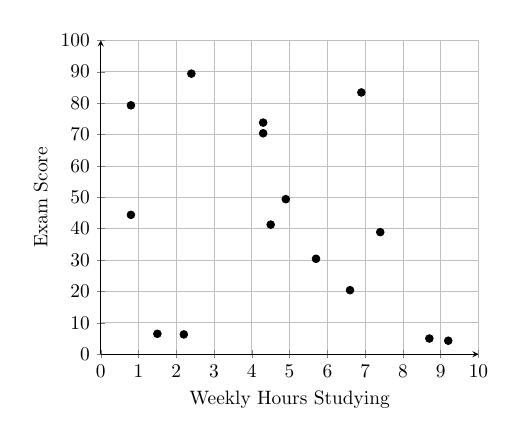
\begin{tikzpicture}[scale=0.7]
	\begin{axis}[
	axis lines = left, grid,
	xlabel = {Weekly Hours Studying},
	ylabel = {Exam Score},
	xmin = 0, xmax = 10,
	ymin = 0, ymax = 100,
	xtick = {0,1,...,10},
	ytick = {0,10,...,100}
	]
	\addplot [only marks] coordinates {(4.9, 49.4)
		(6.9, 83.4)
		(2.4, 89.4)
		(4.3, 73.8)
		(1.5, 6.5)
		(2.2, 6.3)
		(4.3, 70.4)
		(4.5, 41.3)
		(7.4, 38.9)
		(0.8, 79.3)
		(9.2, 4.3)
		(5.7, 30.4)
		(8.7, 5.0)
		(0.8, 44.4)
		(6.6, 20.4)};
	\end{axis}
	\end{tikzpicture}
	\end{center}
}
\end{frame}

\begin{frame}{Line Graph}
A line graph is similar to a scatterplot, however, the points are connected in the order they are obtained.	\newline\\
\begin{center}
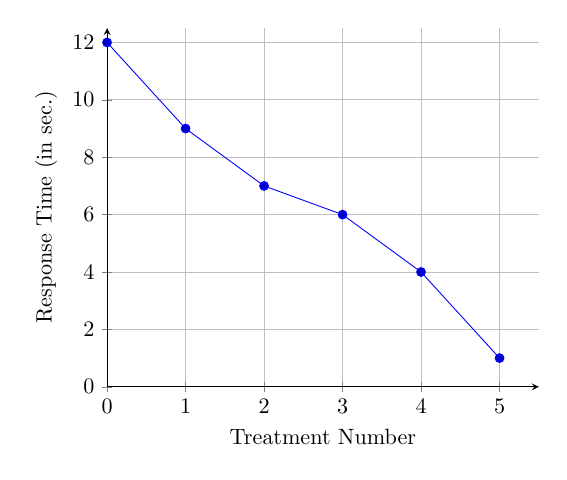
\begin{tikzpicture}[scale=0.8]
\begin{axis}[
	axis lines = left, grid,
	xlabel = {Treatment Number},
	ylabel = {Response Time (in sec.)},
	xmin = 0, xmax = 5.5,
	ymin = 0, ymax = 12.5,
	xtick = {0,1,...,5},
	ytick = {0,2,4,...,12}
	]
	\addplot coordinates {
	(0,12) (1,9) (2,7) (3,6) (4,4) (5,1)
	};
\end{axis}
\end{tikzpicture}
\end{center}
\end{frame}

\begin{frame}{Time Series Graph}
A time series graph is like a line graph, but shows changes over a specific period of time.	\newline\\
\begin{center}
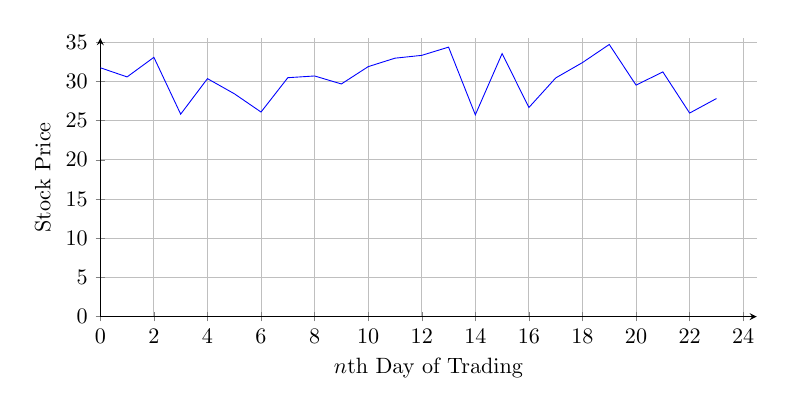
\begin{tikzpicture}[scale=0.8]
\begin{axis}[
	axis lines = left, grid,
	width = 12cm, height = 6cm,
	xlabel = {$n$th Day of Trading},
	ylabel = {Stock Price},
	xmin = 0, xmax = 24.5,
	ymin = 0, ymax = 35.5,
	xtick = {0,2,...,24},
	ytick = {0,5,...,35}
	]
	\addplot [no marks, color=blue] coordinates {
	(0.0, 31.74)
	(1.0, 30.57)
	(2.0, 33.07)
	(3.0, 25.82)
	(4.0, 30.35)
	(5.0, 28.43)
	(6.0, 26.09)
	(7.0, 30.47)
	(8.0, 30.69)
	(9.0, 29.67)
	(10.0, 31.88)
	(11.0, 32.96)
	(12.0, 33.32)
	(13.0, 34.37)
	(14.0, 25.74)
	(15.0, 33.55)
	(16.0, 26.67)
	(17.0, 30.44)
	(18.0, 32.4)
	(19.0, 34.71)
	(20.0, 29.52)
	(21.0, 31.21)
	(22.0, 25.96)
	(23.0, 27.81)
	};
\end{axis}
\end{tikzpicture}
\end{center}
\end{frame}

\section{Examine qualities of misleading graphs}

\begin{frame}{Misleading Graphs}
Some visual displays, whether intentional or not, can be misleading.	\newline\\	\pause

Some things to watch out for are \newline\\	\pause
\begin{itemize}
	\item Vertical axis not starting at 0	\pause
	\item Use of 3 dimensions \pause
	\item Disproportionate use of area
\end{itemize}
\end{frame}

\begin{frame}{Vertical Axis and Zero}
Sometimes, data can be misleading because the vertical axis can be misleading. \newline\\	\pause

Examine the bar graph below. Note that Smith received 53 votes and Jones received 42 votes.
\begin{center}
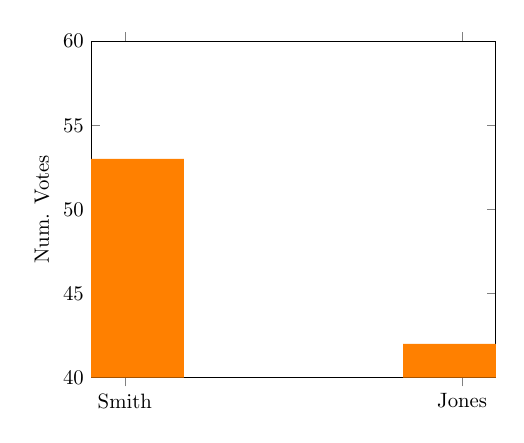
\begin{tikzpicture}[scale=0.75]
\begin{axis}[
ybar, bar width = 2cm,
ymin = 40, ymax = 60, ylabel = {Num. Votes},
symbolic x coords = {Smith, Jones}, xtick=data
]
\addplot [draw=none, fill=orange] coordinates {(Smith,53) (Jones,42)};
\end{axis}
\end{tikzpicture}
\end{center}
\end{frame}

\begin{frame}{Vertical Axis and Zero}
Bar graph with base of 0 for vertical axis:
\begin{center}
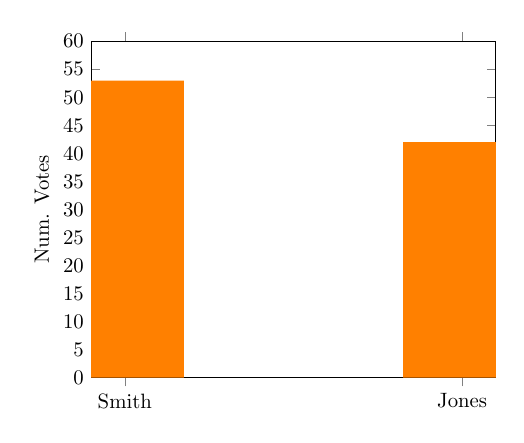
\begin{tikzpicture}[scale=0.75]
\begin{axis}[
ybar, bar width = 2cm,
ymin = 0, ymax = 60, ylabel = {Num. Votes},
ytick = {0,5,...,60},
symbolic x coords = {Smith, Jones}, xtick=data
]
\addplot [draw=none, fill=orange] coordinates {(Smith,53) (Jones,42)};
\end{axis}
\end{tikzpicture}
\end{center}
\end{frame}

\begin{frame}{Use of 3 Dimensions}
Using 3 dimensions for bar graphs or histograms can result in data appearing slightly larger in frequency or relative frequency than it should.	\pause

\begin{center}
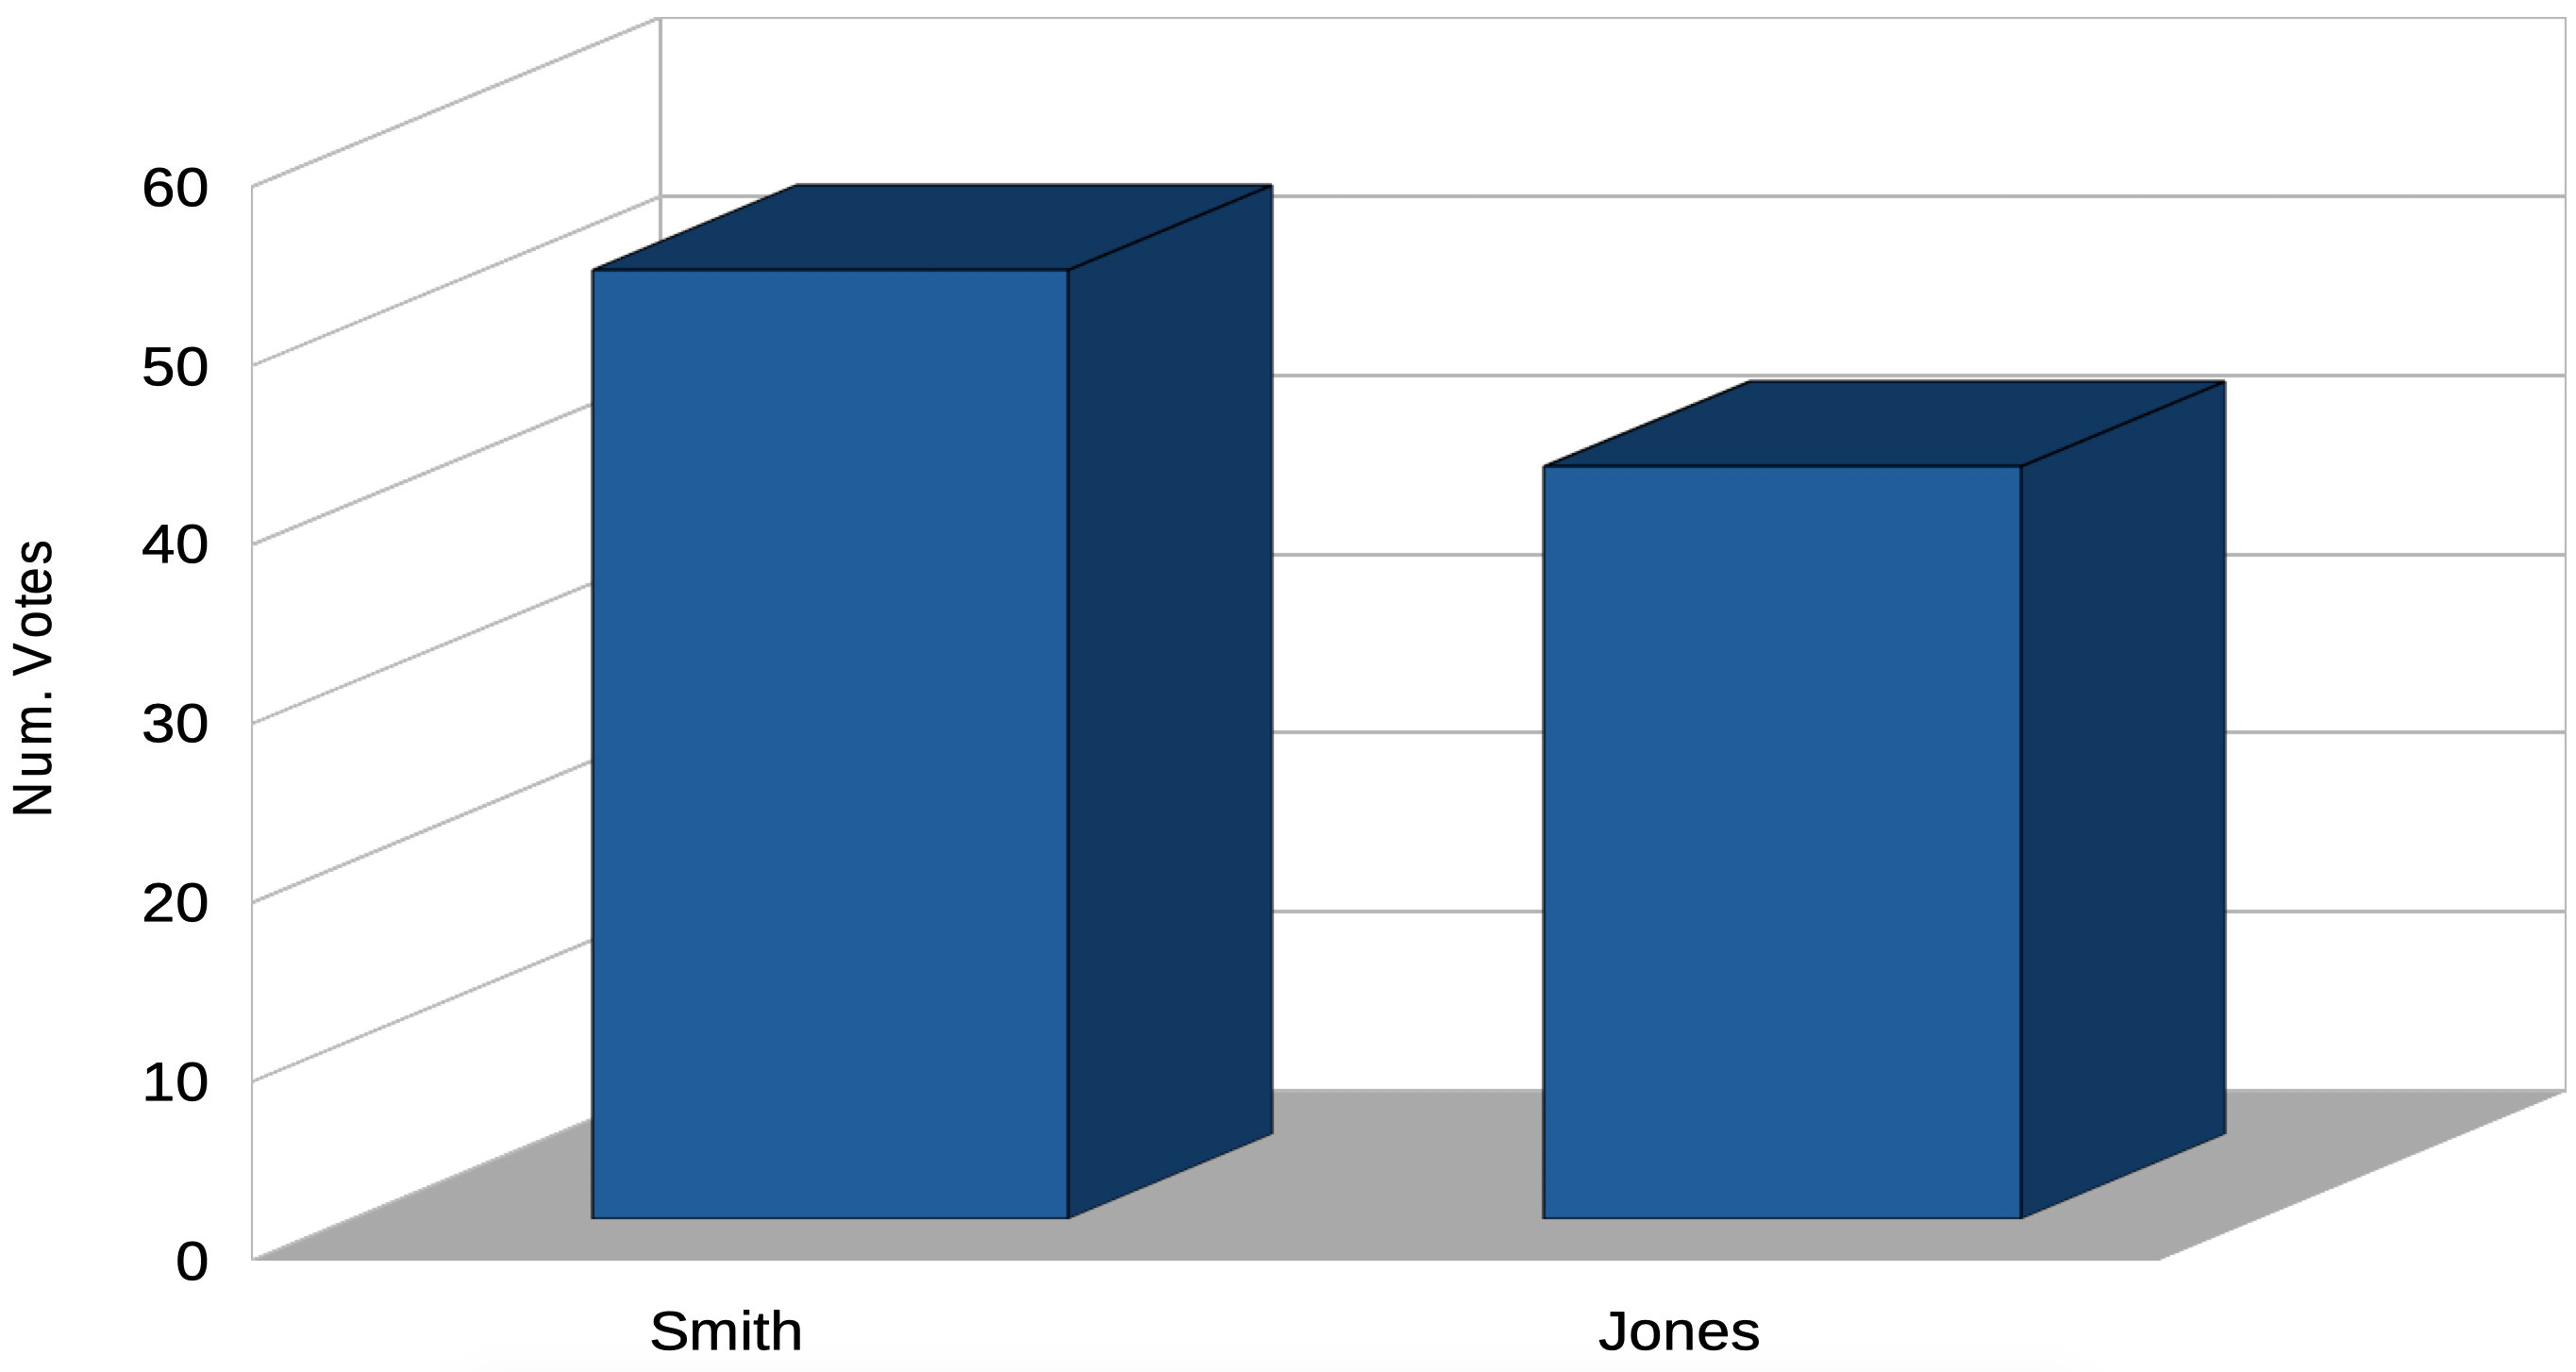
\includegraphics[scale=0.2]{../Images/3D_BarGraph.png}
\end{center}
\end{frame}

\begin{frame}{Disproportionate Use of Area}
Smith received 53 votes and Jones received 42 votes.	\newline\\	\pause

Using bubbles to represent the number of votes each candidate received (Smith radius = 5.3 cm and Jones radius = 4.2 cm) can also be misleading:	\pause

\begin{center}
\begin{tikzpicture}[scale=0.4]
\draw (0,0) circle [radius = 5.3cm] node at (0,0) {Smith};	
\draw (12,0) circle [radius = 4.2cm] node at (12,0) {Jones};
\end{tikzpicture}
\end{center}
\end{frame}

\begin{frame}{More Information on Visual Displays of Data}
\begin{center}
\textit{The Visual Display of Quantitative Information}. Edward R. Tufte. Graphics Press. 2nd ed. 2001	\newline\\
\begin{turn}{-90}
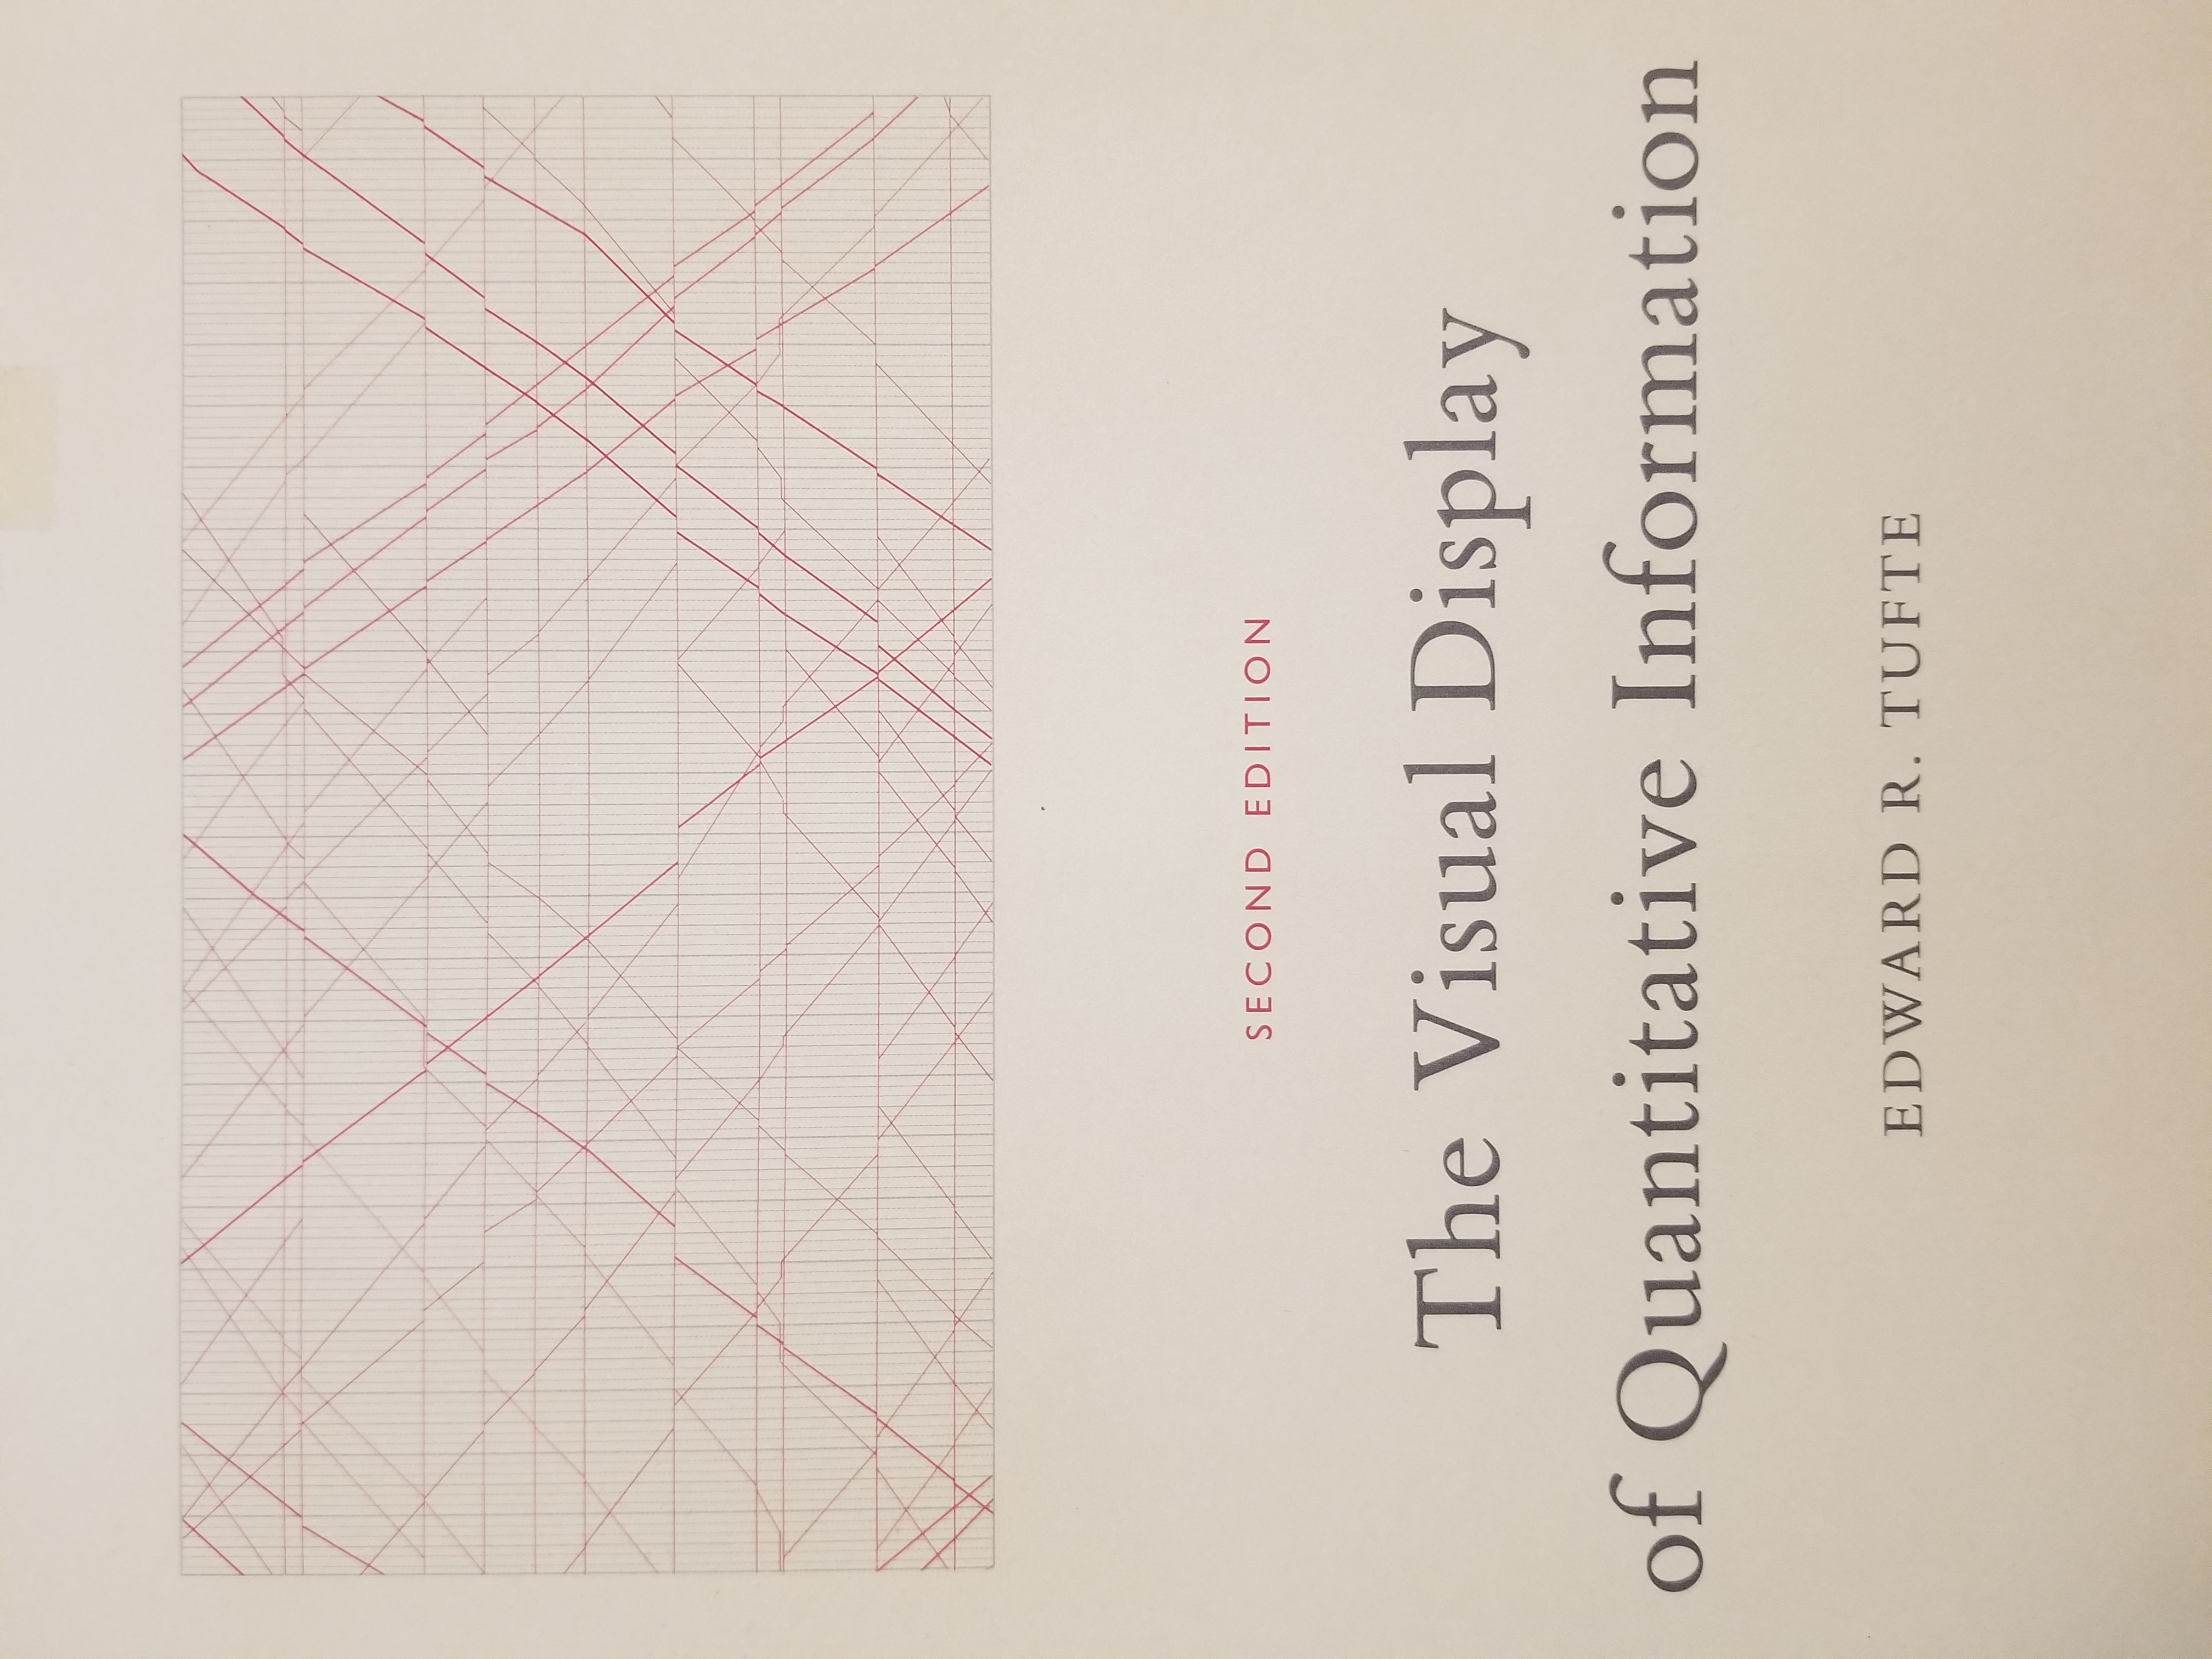
\includegraphics[scale=0.035]{../Images/Tufte.jpg}
\end{turn}
\end{center}
\end{frame}

\end{document}